\documentclass{ijitcs}

\usepackage{amsmath,amssymb,multirow,array}
\usepackage{tikz}
\usepackage{enumerate}
\usepackage{float}

\IjitcsSet{
title = {A Survey of Security and Privacy  in  Cloud Computing: Challenges, Solutions   and Future Directions},
% title = {A Survey of Security and Privacy  in\\ Cloud Computing: Challenges, Solutions \\ and Future Directions},
    volume = {14},
    issue = {6},
    year = {2022},
    month = {December 8},
    startpage = {1},
    endpage = {4},
    doi = {10.5815/ijitcs.2022.06.01},
    abstract = {
       As organizations increasingly transition critical operations to the cloud, ensuring strong security measures becomes paramount. However, the evolving threat landscape poses significant challenges as cyber adversaries continually devise sophisticated tactics to exploit vulnerabilities in cloud infrastructure. This survey paper gives an overview of cloud computing infrastructure, how cloud computing works, as well as how major companies around the world implement cloud computing transformation. The article also provides in-depth analysis of the current threats facing cloud security, from data breaches and insider threats to sophisticated attacks and vulnerabilities in the supply chain. By examining real-world case studies and industry reports, we identify key vulnerabilities that leave cloud environments at risk of exploitation. Furthermore, this article includes the security options offered by the major vendors, thereby exploring the emerging trends and technologies that are shaping the future of cloud security. Additionally, we discuss the role of automation, orchestration, and artificial intelligence in enhancing threat detection and response in the cloud.
    },
    keywords = {cloud computing, attacking vectors, future directions},
    received = {Date Month, Year; Revised: Date Month, Year; Accepted: Date Month, Year; Published: Date Month, Year}
}

\author*{Mai Thanh Duy}{Department of Faculty of Applied Mathematics and Informatics, Hanoi University of Science and Technology, Hanoi, Vietnam}{duy.mt227225@sis.hust.edu.vn}{https://orcid.org/0000-xxxx-xxxx-xxxx}

\author{Tran Duc Toan}{Department of Faculty of Applied Mathematics and Informatics, Hanoi University of Science and Technology, Hanoi, Vietnam}{toan.td195929@sis.hust.edu.vn}{https://orcid.org/0000-xxxx-xxxx-xxxx}

\author{Vu Van Nghia}{Department of Faculty of Applied Mathematics and Informatics, Hanoi University of Science and Technology, Hanoi, Vietnam}{nghia.vv206205@sis.hust.edu.vn}{https://orcid.org/0000-xxxx-xxxx-xxxx}












\thispagestyle{thefirstpage}
\begin{document}


\maketitle


\section{Introduction}
 In recent years, cloud computing has emerged as a dominant paradigm in the realm of IT infrastructure, driven by a confluence of market forces and technological advancements. The dynamic nature of modern business environments has propelled organizations  towards adopting cloud-based solutions to meet their evolving computational needs. With an ever-expanding array of enterprise services and applications, companies are increasingly reliant on cloud infrastructures to support their operations.

 This explores the multifaceted landscape of cloud security, divided into four chapters. In first chapter: Security Issues and Threats,  devilving into the various security concerns that plague cloud environments, examining real-world examples and their implications for cloud security. In Attack Patterns: Understanding the methods and patterns used by attackers is crucial for devising effective security measures. This chapter explores common attack vectors targeting cloud infrastructures, providing insights into malicious strategies. In Current Techniques to Counter: mitigating the risks posed by security threats, organizations deploy a range of techniques and technologies. This chapter reviews the current state-of-the-art approaches for securing cloud environments. Finally, in Future Directions: Looking ahead, the landscape of cloud security is poised for continued evolution. This final chapter examines emerging trends and technologies that are shaping the future of cloud security.

%%%%%%%%%%%%%%%%%%%%%%%%%%%%%%%%%%%%%%%%%%%%%%%%%%%%%%%
\section{Security and Privacy challenges}
In this section, we investigate the specific security and privacy challenges in cloud computing which pose lots of threats, risks and require the development of advanced security technologies.
A “threat” is an act of coercion of a potential attack to elicit negative response. It is generally an effect that can be described as anything that would tamper, destruct or interrupt of any service or item of value. The term “risk” refers to the possibility of being targeted by an attack, getting success and exposed by the attack. The term “vulnerability” refers to the security flaws in a system that allows an attack to be successful . In general, the threats exploit the vulnerabilities of a system, which leads to risk by damaging assets and causing exposure. However, threats can be identified in order to mitigate risks and countermeasure for vulnerabilities.

\subsection{Loss of control}
\subsubsection{Data Loss and Data Theft}
Data loss and data breaches were recognized as the top threats in cloud computing environments in 2013. A recent survey shows that 63\% of customers would be less likely to purchase a cloud service if the cloud vendor reported a material data breach involving the loss or theft of sensitive or confidential personal information.Whether a C can securely maintain customers’ data has become the major concern of cloud users. The frequent outages occurring on reputable CSPs, including Amazon, Dropbox, Microsoft, Google Drive, \dots, further exacerbate such concerns \cite{liu2015survey}.

\textbf{Data Loss:} Due to the number of interactions between known/unknown risks \& challenges in the architectural or operational characteristics of Cloud Computing. Accidental deletion or alteration of records without a backup; Storage on unreliable media; Loss of encoding key by customer; unauthorized access to sensitive data; operational failures; disposal challenges; risk of association; jurisdiction \& political issues; data centre reliability; physical catastrophe; disaster recovery; Results: devastating business impact; damage to brand \& reputation; impact stakeholders’ moral \& trust; loss of property; leakage of data lead to compliance violations \& legal ramifications \cite{ahmad2017cloud}.

\textbf{Data theft:} In a multitenant infrastructure, if cloud service database has error in design, a flaw in one client’s application will allow an attacker to access not only to that application data but every others’ data as well. Offline backups of data to avoid catastrophic data loss will also increase the chance of exposure to data breach \cite{ahmad2017cloud}.

\subsubsection{Data storage and tranmission through regional norms}
Due to the distributed infrastructure of the cloud, cloud users’ data may be stored on data centers geographically located in multiple legal jurisdictions, leading to cloud users’ concerns about the legal reach of local regulations on data stored out of region. Furthermore, the local laws may be violated since the dynamic nature of the cloud makes it extremely difficult to designate a specific server or device to be used for transborder data transmission \cite{liu2015survey}.

\subsubsection{Cheap Data Leakage and Analysis}
The rapid development of cloud computing has facilitated the generation of big data, leading to cheap data collections and analysis. For example, many popular online social media sites, such as Facebook, Twitter and LinkedIn, are utilizing the cloud computing technology to store and process their customers’ data. Cloud providers that store the data are gaining considerable business revenue by either retrieving user information through data mining and analysis by themselves or selling the data to other businesses for secondary usage. One example is that Google is using its cloud infrastructure to collect and analyze users’ data for its advertisingnetwork.
Such data usage has raised extensive privacy concerns since the sensitive information of cloud users may be easily accessed and analyzed by unauthorized parties. The Electronic Privacy Information Center (EPIC) asked to shut down Gmail, Google Docs, Google Calendar, and the company’s other Web apps until government-approved
“safeguards are verifiably established”. Netflix had to cancel its \$1 million data challenge prize due to a legal suit because it violated customers’ privacy during the data sharing process. While technologies such as data anonymization are under investigation, users’ data privacy has to be fundamentally protected by standards, regulations and laws \cite{liu2015survey}.

\subsection{Shortage of Transparency}
\subsubsection{Malicious Insiders/Unauthorized Internal Access}
Threats amplify due to the convergence of IT services under a single management domain; General lack of transparency into CSP processes \& procedures; less visibility into the hiring standard and practices of cloud employees’ lead to adversary. A malicious insider, such as a system administrator, in an improperly designed cloud scenario can have access to potentially sensitive information. Results: Espionage; hacker; organized crime; corporate espionage; spoofing; tampering, information disclosure; nation-state sponsored intrusion; Brand damage; financial impact; productivity losses; impact on business continuity, traditional security and disaster recovery \cite{ahmad2017cloud}.

\subsubsection{Ambiguous ownership \& responsibility}
Lack of clear ownership and defined responsibilities for data protection may responsibility result in failure of meeting regulatory and of data legal obligations \cite{ahmad2017cloud}.

\textbf{Authentication \& Authorization:} Cloud building organizations has to authenticate each and every person who is using the cloud from the cloud utilizing organization. They will provide authorizations to the users based on the service usage and payment. The cloud building organization has to prevent unauthorized users by checking authorization. The cloud utilizing organization has to remove or disable accounts of the ex-employees on day-to-day basis \cite{mandala2012cloud}.

\subsection{Virtual Machine Related Challenges}
Virtualization refers to the logical abstraction of computing resources from physical constraints. One representative example of virtualization technology is the virtual machine (VM). Virtualization can also be performed on many other computing resources, such as operating system, networks, memory, and storage. In a virtualized environment, computing resources can be dynamically created, expanded, shrunk or moved according to users’ demand, which greatly improves agility and flexibility, reduces costs and enhances business values for cloud computing.

Despite of its substantial benefits, this technology also introduces security and privacy risks in the cloud computing environment.

\subsubsection{Security threats sourced from host}
Monitoring VMs from host The control point in virtual environment is the host machine there are implications that allow the host to monitor and communicate with VM applications up running. Therefore, it is more necessary to strictly protect the host machines than protecting distinctive VMs . VM-level protection is crucial in cloud computing environment. The enterprise can co-locate applications with different trust levels on the same host and can defend VMs in a shared multi-tenant environment. This enables enterprises to maximize the benefits of virtualization. VM-level protection allows VMs to stay secure in today’s dynamic data centers. Also, as VMs travel between different environments – from on-premise virtual servers to private clouds to public clouds, and even between cloud vendors
\cite{hussein2016survey}.

Communications between VMs and host The data transfer between VMs and the host flow between VMs shared virtual resources; in fact the host can monitor the network traffic of its own hosted VMs. This can be considering useful features for attackers and they may use it such as shared clipboard which allows data to transfer between VMs and the host using cooperating malicious program in VMs. It is not generally considered a bug or limitation when one can initiate monitoring, change, or communication with a VM application from the host. The host environment needs to be more strictly secured than the individual VMs. The host can influence the VMs in the following ways \cite{hussein2016survey}:

\begin{itemize}
\item The host can Start, shutdown, pause, and restart VMs.
\item Monitoring and configuration of resources which are available to the VMs, these include: CPU, memory, disk, and network usage of VMs.
\item Adjust the number of CPUs, the amount of memory, the amount and number of virtual disks, and a number of virtual network interfaces which are available to a VM.
\item Monitoring the applications which are running inside the VM.
\item View, copy, and possibly modify, data stored on the VM's virtual disks. Unfortunately, the system admin or any authorized user who has privileged control over the backend can misuse these procedures.
\end{itemize}

\subsubsection{Security threats sourced from other VM}

\textbf{Monitoring VMs from other VM:} Monitoring VMs could violate security and privacy, but the new architecture of CPUs, integrated with a memory protection feature, could prevent security and privacy violation. A major reason for adopting virtualization is to isolate security tools from an untrusted VM by moving them to a separate trusted secure VM.

\textbf{Communication between VMs:} One of the most critical threads that threaten exchanging information between virtual machines is how it's deployed. Sharing resources between VMs may strip security of each VM for instance collaboration using application such as shared clipboard that allow exchanging data between VMs and the host assisting malicious program in VMs, this situation violate security and privacy. Also, a malicious VM can has chance to access other VMs through shard memory.

\textbf{Denial of Service (DoS):} A DoS attack is a trying to denial services that provide to authorize users. For example when trying to access site we see that due to overloading of the server with the requests to access the site, we are unable to access the site and observe an error. This happens when the number of requests that can be handled by a server exceeds its capacity, the Dos attack marking carting part of clouds inaccessible to the users. Usage of an Intrusion Detection System (IDS) one of the useful method of defense against this type of attacks.

\subsection{Managerial Issues}
Most cloud-specific security and privacy challenges have their own managerial aspect. For example, the malicious insider challenge involves the problem of effectively managing employees to detect early warning signs and responding to policy violations in a timely manner once malicious insider incidents occur. These managerial challenges are non-technical in nature but also closely related to the technical solutions that could help cope with the corresponding technical challenges.

Implementing a technical solution and not managing it properly are bound to introduce vulnerabilities. For example, security management for virtualization, which is dramatically unlike that of traditional networks, requires knowledge and skill sets beyond the capabilities of the general network administrator, leading to increased management complexity and risks. Inappropriate VM management policies may cause the number of VMs to continuously grow while most of them are in the middle or sleep mode leading to the host machine’s resource exhaustion.

The fact that managerial challenges are overarching and add to the other challenges is what makes it one of the toughest challenges to deal with. CSPs have to make a decision on the scope of their managerial effort in order not to exhaust their resources before all their most critical security and privacy goals and objectives are met \cite{liu2015survey}.

%%%%%%%%%%%%%%%%%%%%%%%%%%%%%%%%%%%%%%%%%%%%%%%%%%%%%%%
\section{Attacking vectors}
%%%%%%%%%%%%%%%%%%%%%%%%%%%%%%%%%%%%%%%%%%%%%%%%%%%%%%%
\subsection{Brute-Force Attacks}

A brute-force attack consists of an attacker submitting many passwords or passphrases with the hope of eventually guessing correctly.
The attacker systematically checks all possible passwords and passphrases until the correct one is found. Alternatively, the attacker can attempt to guess the key which is typically created from the password using a key derivation function.
This is known as an exhaustive key search.
In theory, be used to attempt to decrypt any encrypted data (except for data encrypted in an information-theoretically secure manner). Such an attack might be used when it is not possible to take advantage of other weaknesses in an encryption system (if any exist) that would make the task easier\cite{kanakam2022bruteforce}.
%%%%%%%%%%%%%%%%%%%%%%%%%%%%%%%%%%%%%%%%%%%%%%%%%%%%%%%
\subsection{Distributed Denial of Service - DDoS Attack}
\subsubsection{What is DDoS?}
\par DDoS \cite{coppolino2017cloud} is one of the Network-Based Attacks, which come from the Internet. The network is one of the main vehicles of attacks against applications running on a cloud platform. Most of these attacks are direct descendants of attacks initially conceived for traditional technology, some were invented after the birth of cloud computing technology. Zargar\cite{coppolino2017cloud} made an exhaustive classification of DDoS flooding attacks, dividing them into two types based on the protocol level that they targeted: network/transport level and application level attacks. DDoS attacks are launched by affecting the victim in the following forms:

\begin{itemize}
\item Attackers can find some bug or weakness in the software implementation to disrupt the service.
\item Some attacks deplete all the bandwidth or resources of the victims' system.
\end{itemize}
Attackers scan the network to find the machines which have some vulnerability. Then, the attacker uses these as agents, called zombie machines. Zombie machines use spoofed IPs. The design of the internet gives rise to many conditions causing denial of service attacks. Security on the internet is dependent on hosts. Attackers compromise the security of hosts to launch DDoS
attacks and use spoofed IP addresses making it difficult to trace attack source. Further internet is full of hosts. It
gives attackers various options, out of which vulnerable hosts are chosen\cite{deshmukh2015understanding}. Although widely known as a method of clogging transmission lines between servers on the Internet, DDoS seems to be more dangerous than people thought. In the past, many large-scale, highly complex attacks related to DDoS had been carried out. Those attacks can target finance, can also delay major events, put pressure on agencies, companies or famous websites. The attacks in 2013 include the attack on China’s websites, Bitcoin, the largest cyber-attack by Cyber Bunker, the NASDAQ trading market, Iranian Cyber-attacks on FBI and so on. From the above survey, most of the victims of DDoS
attacks are distributed and shared. Apart from the list mentioned, numerous anonymous tools are emerging daily. Here is the list of the DDoS attacks that occurred over the years and how they evolved.
\begin{itemize}
    \item In 1998, the first DDoS tools were discovered.
    \item In 1999, the University of Minnesota was attacked, and the network was unusable for more than 2 days.
    \item In 2000, Yahoo’s website became victim of an attack.  CNN, eBay, Dell, Amazon, and many other major websites were also shown to be feasible before a DDoS attack.
    \item 2001 witnessed a tremendous transformation in the size of DDoS attack. The attack size grew from Mbps to Gbps.
    \item In August of 2005, jaxx.de, a gambling site was under DDoS attack and to stop this attack, the attacker demanded 40,000 euros.
    \item In December 2007 during the riots in Russia, government sites suffered severe DDoS attacks. Access to IP addresses outside Estonia was removed for several days.
    \item In November 2008, the Conficker worm used vulnerabilities found in Microsoft OS. It uses vulnerable machine and other machines are unwillingly connected to it, to make a large botnet.
    \item On 4th July (Independence Day in the US) 27 websites of White House, Federal Trade Commission, Department of Transportation, and the Department of the Treasury were attacked. On 1st august, Blogging pages of many social networking sites (Twitter, Facebook etc.) were affected by DDoS attack, aimed at “Cyxymu” Georgian blogger.
\end{itemize}

\subsubsection{DDoS Constituents}
% \begin{figure}[H]
\begin{figure}[h]
    \centering
    % \includegraphics{pictures/Attacking_vectors/Consistent.PNG}
\includegraphics[scale = 1]{pictures/Consistent.PNG}
    \caption{Consistent of DDoS attack}
    \label{fig:consistnt}
\end{figure}
Recently, Botnets are been used widely to perform DDoS attacks. This section explains botnet architectures and
the tools that have been used to launch DDoS flooding attacks. Many computers are used for launching a DDoS
Attack. It makes use of client-server technology. In general, DDoS attack comprises of Master, Handler, Agents and
victim. The zombies (agents or bots) are the ones used by the master to form a botnet. The larger the number of zombies, the more disruptive the attack will be. The Master communicates with agents via handlers. For example, handlers can be programs installed on a set of compromised devices (e.g., network servers) that attackers communicate with to send commands. Attacker sends commands and controls their agent through handlers. Bots are
devices that the handlers have compromised.
The bots attack the victim’s system. Attacker uses many scanning techniques to find a vulnerable machine.
Random Scan is the simplest strategy which randomly scans whole IPv4 address space as the worm doesn’t know
where the host is present. It is effective only for IPv4 as the address space of IPv6 is too vast. Hitlist Scan has a
list that contains IP address vulnerable hosts on the Internet. The scanning is done in this list. When it makes
another machine a host, part of the initial hit list will be sent to that machine. Route-based Scan reduces the search
addresses BGP routing prefixes are used and this prefixes information can reduce the search space drastically. In
Divide-and-conquer Scan technique the scanning is done by different hosts on different parts of address space hence
saving resources. Apart from these, there are other strategies too like Permutation Scan, Local Preference Scan
and Topological Scan. Once host is found after scanning, vulnerabilities of that host need to be found to gain its
control\cite{deshmukh2015understanding}. 
\subsubsection{DDoS Classification}.
In today's digital world, the internet is not only a place for information exchange but has also become a large environment for cyber attacks. Among common types of attacks, distributed denial of service (DDoS) attacks are one of the most dangerous and complex. To better understand how DDoS attacks work, we need to look deeper into the types of attacks and how they affect the network environment. The variety of DDoS attacks are sprouting in the computing world. The major types include Bandwidth based and
resource-based attacks. Both types consume the entire bandwidth and resources of the network.
% \begin{figure}[H]
%     \centering
%     \includegraphics{pictures/Attacking_vectors/Classification.PNG}
%     \caption{Taxonomy of DDoS Attacks}
%     \label{fig:Calssification}
% \end{figure}

\begin{figure}[h]
\centering

    \resizebox{0.3\textwidth}{!}{%
     
    \tikzset{every picture/.style={line width=0.75pt}} %set default line width to 0.75pt        

    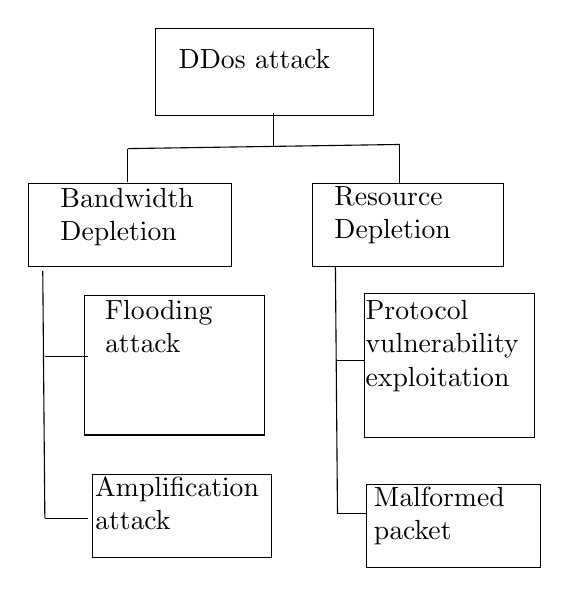
\begin{tikzpicture}[x=0.75pt,y=0.75pt,yscale=-1,xscale=1]
        %uncomment if require: \path (0,300); %set diagram left start at 0, and has height of 300
    
        %Shape: Rectangle [id:dp7909079015892935] 
        \draw   (403,33.08) -- (508.16,33.08) -- (508.16,75) -- (403,75) -- cycle ;
        %Shape: Rectangle [id:dp31644531544911914] 
        \draw   (341.76,108) -- (439.76,108) -- (439.76,148) -- (341.76,148) -- cycle ;
        %Shape: Rectangle [id:dp8856914330072934] 
        \draw   (478.76,108) -- (570.76,108) -- (570.76,148) -- (478.76,148) -- cycle ;
        %Shape: Rectangle [id:dp6364353066973951] 
        \draw   (503.76,161) -- (585.76,161) -- (585.76,230.08) -- (503.76,230.08) -- cycle ;
        %Shape: Rectangle [id:dp43831551281650505] 
        \draw   (368.76,162) -- (455.76,162) -- (455.76,229.08) -- (368.76,229.08) -- cycle ;
        %Straight Lines [id:da5415287891795697] 
        \draw    (459.76,74.08) -- (459.76,90.08) ;
        %Straight Lines [id:da9353308432304241] 
        \draw    (389.76,91.08) -- (520.76,89.08) ;
        %Straight Lines [id:da022067968769266644] 
        \draw    (389.76,91.08) -- (389.76,107.08) ;
        %Straight Lines [id:da9073360600243896] 
        \draw    (520.76,89.08) -- (520.76,108.08) ;
        %Shape: Rectangle [id:dp49507696721847827] 
        \draw   (504.76,253) -- (588.76,253) -- (588.76,293) -- (504.76,293) -- cycle ;
        %Shape: Rectangle [id:dp22439615778259836] 
        \draw   (372.76,248) -- (458.76,248) -- (458.76,288) -- (372.76,288) -- cycle ;
        %Straight Lines [id:da2743840804903954] 
        \draw    (348.76,150.08) -- (349.76,269.08) ;
        %Straight Lines [id:da7751224415151379] 
        \draw    (489.76,148.08) -- (490.76,267.08) ;
        %Straight Lines [id:da011605619201682682] 
        \draw    (349.76,191.08) -- (370.76,191.08) ;
        %Straight Lines [id:da915007187431224] 
        \draw    (349.76,269.08) -- (370.76,269.08) ;
        %Straight Lines [id:da671418896264715] 
        \draw    (504.76,267.08) -- (490.76,267.08) ;
        %Straight Lines [id:da612764489223284] 
        \draw    (503.76,193.08) -- (490.76,193.08) ;
    
        % Text Node
        \draw (413,42) node [anchor=north west][inner sep=0.75pt]   [align=left] {DDos attack};
        % Text Node
        \draw (356,109) node [anchor=north west][inner sep=0.75pt]   [align=left] {Bandwidth\\Depletion};
        % Text Node
        \draw (488,108) node [anchor=north west][inner sep=0.75pt]   [align=left] {Resource\\Depletion};
        % Text Node
        \draw (503.05,163) node [anchor=north west][inner sep=0.75pt]   [align=left] {Protocol\\vulnerability\\exploitation};
        % Text Node
        \draw (377.56,163) node [anchor=north west][inner sep=0.75pt]   [align=left] {Flooding \\attack};
        % Text Node
        \draw (507.05,253) node [anchor=north west][inner sep=0.75pt]   [align=left] {Malformed\\packet};
        % Text Node
        \draw (372.76,248) node [anchor=north west][inner sep=0.75pt]   [align=left] {Amplification\\attack};
    
    
    \end{tikzpicture}
    
    }
     \caption{Taxonomy of DDoS Attacks}
    \label{fig:Calssification}
    \end{figure}

\textbf{Bandwidth Depletion Attacks:} This type of attack consumes the bandwidth of the victim or target system by flooding the unwanted traffic to prevent the legitimate traffic from reaching the victim network. Bandwidth depletion attacks are categorized further as:
\begin{itemize}
    \item \textbf{Flood Attacks:} This attack is launched by an attacker sending a huge volume of traffic to the victim with the help of zombies that clog up the victim’s network bandwidth with IP traffic. A flood attack is initiated by UDP (User Datagram packets) and ICMP (Internet Control Message Protocol), with the following UDP attack steps\cite{deshmukh2015understanding}:
    \begin{enumerate}
        \item An attacker sends a large number of UDP packets to the victim system’s random or specified ports with the help of zombies.
        \item On receiving the packets, the victim system looks the destination ports to identify the applications waiting on the port.
        \item When there is no application, it generates an ICMP packet with a message “destination unreachable”.
        \item The return packets from the victim are sent to the spoofed address and not to the zombies.
    \end{enumerate}
    and ICMP attack steps\cite{deshmukh2015understanding}:
    \begin{enumerate}
        \item An attacker sends a large number of ICMP ECHO REPLY i.e. ping packets to the victim system with the help of zombies. This kind of packets requires a response message from the victim.
        \item The victim sends the responses to the packets received.
        \item Now the network is clogged with request response traffic. The spoofed IP address may be used in the ICMP packet.
    \end{enumerate}
    As a result the available bandwidth has been depleted without servicing the legitimate users. This impacts the
connections and systems located near the victim. Other variations of this attack include Fragmentation, DNS
flood attack, VoIP flood attack, Media data flood attack, etc...
    \item \textbf{Amplification attacks:} This is a type of DDoS attack that uses the IP broadcast protocol. The attacker sends packets to the broadcast address, causing systems within that address range to respond to the victim's system, generating malicious network traffic. This type of attack takes advantage of the broadcast address feature in network devices such as routers. This can be done directly by the attacker or through control of the clients. Typical examples of this type of attack include Smurf and Fraggle attacks. The Smurf attack is caused by the following steps\cite{deshmukh2015understanding}:
    \begin{enumerate}
        \item Attacker sends packets to a network device that supports broadcast addressing technique. The return address in these packets are forged or spoofed with victim’s address.
        \item ICMP ECHO RESPONSE packets are sent by the network amplifier to all the systems in the broadcast IP address range. This packet implies the receiver to respond with an ICMP ECHO REPLY.
        \item An ICMP ECHO REPLY message from all the systems in the range reaches the victim.
    \end{enumerate}
    and the Fraggle one\cite{deshmukh2015understanding}:
    \begin{enumerate}
        \item Attacker sends UDP echo packets to a port that supports character generation. The return address in these packets is forged or spoofed with victim’s address with the port supporting character generation thus creating an infinite loop.
        \item This targets the port supporting character generation of all the systems reached by broadcast address.
        \item All these systems in the range echo back to the character generator port in the victim.
        \item This process repeats since UDP echo packets are used.
    \end{enumerate}
    This attack is worse than the Smurf attacks. Reflector, a variation of Smurf attacks, uses intermediary servers, called reflectors, to increase the power of the attack. Reflector continues to respond to the packets it receives, and the attacker uses them to attack the target by spoofing the target's IP address.
\end{itemize}
\textbf{Resource Depletion Attacks:} The DDoS Resource depletion attack is targeted to exhaust the victim system’s resources, so that the legitimate users are not serviced. The following are the types of Resource depletion attacks:
\begin{itemize}
    \item \textbf{Protocol Exploit Attacks:} The goal of these attacks is to consume the surplus quantity of resources from the victim by exploiting the specific feature of the protocol installed in the victim. TCP SYN attacks are the best example of this type. The other examples of Protocol exploit attacks are PUSH + ACK attack, authentication server attack and CGI request attack.
    \item \textbf{Malformed Packet Attacks:} The term malformed packet refers to the packet wrapped with malicious information or data. The attacker sends these packets to the victim to crash it. This can be performed in two ways: 
    \begin{itemize}
        \item[] \textbf{IP Address attack:} The malformed packet is wrapped with same source and destination IP address thus creating chaos in the operating system of victim. By this way it rapidly slows down and crashes the victim.
        \item[] \textbf{IP packet options attack:} Each of the IP packets consists of the optional fields to carry additional information. This attack makes use of these fields to form the malformed packet. The optional fields are filled by setting all the quality of service bits to one. So the victim spends additional time to process this packet. This attack is more vulnerable when attacked by more than one zombie.
    \end{itemize}
\end{itemize}

%%%%%%%%%%%%%%%%%%%%%%%%%%%%%%%%%%%%%%%%%%%%%%%%%%%%%%%
\subsection{Insider Threats}

 Security threats can come from inside or outside of an organization. The attacks from insiders, be they from employees, suppliers, or other companies legitimately connected to a company’s computer system, pose a more pernicious threat than external attacks. These insiders have knowledge of the internal workings of the organization, and full possession of all the rights and privileges required to mount an attack that outsiders lack. Consequently, insiders can make their attacks look like normal operations \cite{gheyas2016detection}.

To solve this problem, the goal is to classify knowledge organizations within the scope of threat research. By applying machine learning algorithms and analyzing large-scale studies on detecting internal threats, the development involves classifying current internal personnel into different categories, levels of access rights, and the motivations behind them.

\subsubsection{Classification results}

According to research \cite{singh2022systematic}, by passing keywords to the search engine. The Boolean AND and OR were used to conduct the search. The search terms were: Insider Threats, Insider Threat Detection, Computer Threats, Security. The platforms searched were: IEEE Xplore Digital Library, ScienceDirect, SpringerLink, ACM Digital Library, Google Scholar. With the following criteria:


\begin{itemize}
    \item  Inclusion Criteria
    
\begin{itemize}
    \item   The paper should focus on the insider threats and its types.
    \item    The paper should highlight the insider detection techniques.
    \item     The paper should focus on insider threats challenges and its prevention.
\end{itemize}

    \item Exclusion criteria

    
\begin{itemize}
    \item   The papers should not be about types of threats, it should focus only on insider threats to the cyber world.
    \item    Papers published after 2020.
    \item     The paper should focus on insider threats challenges and its prevention.
\end{itemize}
\end{itemize}



Summary of results received\cite{singh2022systematic}:


\begin{figure}[H]
\centering
\includegraphics[scale = 0.6]{pictures/Summary_of_results_Insider_Threats.png}
    \caption{Summary of results Insider Threats} 
    \label{fig:Summary_of_results_Insider_Threats}
\end{figure}

    
\begin{itemize}
    \item   All the papers has basic information about threat types and its detection.
    \item    It is clear from Fig \ref{fig:Summary_of_results_Insider_Threats}, that majority of studies were focused on threat detection and threat mitigation in insider threats.
    \item     Fig  \ref{fig:Summary_of_results_Insider_Threats}, shows the graphical representation of subdivided categories and their applications in insider threats.
    \item      The themes found in primary studies shows   that threat detection and threat mitigation are the most popular security application in insider threats, with both comprising of 35 percent each respectively.
    \item    The third most popular among the primary studies was, modeling human behaviors to detect the insider threat attack (behavior model). It comprises of 19 Percent of the total studies.
    \item     At the last comes the types of threat, which makes up 11 Percent of the total studies.
\end{itemize}


 




%# \subsubsection{Detection and Protection System}
\subsubsection{Detection System}


To detect the intrusion, an Intrusion Detection System (IDS) is used. To detect the intrusion and respond in timely manner is its prime function.


Based on the deployment IDS broadly classified into 2 types: Host based Intrusion Detection System (HIDS) and Network based Intrusion Detection System (NIDS).  Here is an overview of the two types \cite{leu2015internal}:     

\begin{itemize}
    \item  Host based Intrusion Detection System is configured on a particular system/server. It continuously monitor and analyzes the activities the system where it is configured. Whenever an intrusion is detected HIDS triggers an alert.
    
  \textbf{For instance}, when an attacker tries to create/modify/delete key system files alert will be generated. Major advantages of the HIDS that it analyzes the incoming encrypted traffic which cannot be detected NIDS. To detect the attack like Denial of Service (DoS) attacks, Port Scans, Distributed Denial of Service (DDoS) attack, \dots
  
    \item    Network Intrusion Detection System (NIDS) continuously monitor and analyze the network traffic. To classify as malicious or non-malicious traffic it examines the incoming network traffic. If any predefined patterns or signatures of malicious behavior are present it re-assembles the packets, examine the headers/payload portion and determine.
\end{itemize}

%%%%%%%%%%%%%%%%%%%%%%%%%%%%%%%%%%%%%%%%%%%%%%%%%%%%%%%
\subsection{Malware}
Software that accomplishes deliberately the harmful purpose of an attacker is commonly known as malicious software or malware. Malware is a generic term that
used to describe many types of malicious software, such as viruses and worms.
This section discusses the purpose, categories and vulnerabilities of malware attacks in the wireless networks \cite{divya2013survey}.
%%%%%%%%%%%%%%%%%%%%%%%%%%%%%%%%%%%%%%%%%%%%%%%%%%%%%%%
\subsubsection{Purpose of malware}
The purpose of Malware is to cause damage or penetrate users computer for the purpose of hacking personal data for illegal activity such as financial crimes. Many DoS viruses, and the
Windows Explore Zip worm, are designed to demolish files on a hard disk, or to corrupt the file system by writing void data to them. Profit category of malware develop spyware that are programs designed to monitor display unsolicited advertisements, users' web browsing, or
redirect affiliate marketing revenues to the spyware creators  \cite{divya2013survey}.
%%%%%%%%%%%%%%%%%%%%%%%%%%%%%%%%%%%%%%%%%%%%%%%%%%%%%%%
\subsubsection{Categories of Malware}
 

% \begin{figure}[H]
% \begin{adjustwidth}{-\extralength}{0cm}
% \centering
% \includegraphics[width=22cm]{pictures/Attacking_vectors/malwarecategories.png}
% \end{adjustwidth}
% % \caption{This is a wide figure.\label{fig2}}
% \end{figure}  




\begin{table}[h]
    \centering
    \resizebox{\textwidth}{!}{
        \begin{tabular}{|c|c|c|c|c|}
            \hline
            \textbf{Malwares}                                                & \textbf{Infection}   & \textbf{Through} & \textbf{Types} & \textbf{Prevent} \\
            \hline
            Virus                                                            &   $\begin{array}{l}     \text{Slows down} \\ \text{host computer}  \\ \text{and destruct}  \\ \text{program files and}  \\ \text{system hardware}   \end{array}$   &  $\begin{array}{l}\text{Internet Download,} \\ \text{Attachment in Emails,}  \\ \text{File Sharing Network}   \end{array}$    &  $\begin{array}{l}\text{Boot sector virus,} \\ \text{Polymorphic virus,}   \\ \text{Macro virus,}   \\ \text{Stealth virus,}   \\ \text{Retro virus}   \end{array}$  &  $\begin{array}{l}\text{Anti-virus software} \\ \text{current updates} \\ \text{Periodic System scan}   \end{array}$       \\
            \hline
            Worms                                                            &  $\begin{array}{l}      \text{High bandwidth } \\ \text{Consumption} \\ \text{Web browser } \\ \text{irregularity} \\ \text{OS and System} \\ \text{error Fault}    \end{array}$   & $\begin{array}{l}    \text{Email,} \\  \text{Instant Messaging,} \\  \text{Relay Chats,} \\  \text{File Sharing}     \end{array}$   & $\begin{array}{l}   \text{Conficer,} \\    \text{Black worm,} \\    \text{Morris wom,} \\    \text{XSS, Ramnit worm,} \\    \text{Blaster wom}   \end{array}$  &  $\begin{array}{l}        \text{Updated  firewall and} \\    \text{Antivirus software} \\    \text{Update of} \\    \text{OS and Software}   \end{array}$       \\
            \hline  
            $\begin{array}{l}\text{Trojan} \\  \text{Horses}   \end{array}$   &  $\begin{array}{l}        \text{System crash}   \\ \text{Keystroke logging}   \\ \text{Passwords and}   \\ \text{credit card theft}     \end{array}$    & $\begin{array}{l}        \text{MP3 files,}   \\ \text{image games,}   \\ \text{Movies}     \end{array}$    & $\begin{array}{l}        \text{Netbus, Vundu,}   \\ \text{Zlob Trojan,}   \\ \text{Beast, Zeus,}   \\ \text{Coreflood}     \end{array}$   & $\begin{array}{l}        \text{Anti - virus software}   \\ \text{Anti - Trojan Programs}     \end{array}$         \\
            \hline
            $\begin{array}{l}\text{Blended} \\  \text{Attacks}   \end{array}$ &  $\begin{array}{l}              \text{Damage network}     \\          \text{at a same time}     \\          \text{Disrupts exe files,}     \\          \text{HTML file and registry keys}         \end{array}$    & $\begin{array}{l}           \text{E-Mail,}         \\          \text{IRC,}         \\          \text{File sharing Network}             \end{array}$    & $\begin{array}{l}          \text{Morris worm,}                        \\       \text{Win 32/Nimda A@mm,}                        \\       \text{Win 32/Bolzano,}                        \\       \text{VBS/Bubbleboy}   \end{array}$   & $\begin{array}{l}          \text{Memory scanner}                        \\       \text{solutions}                        \\       \text{Host-based IDS}                        \\       \text{solutions}                        \end{array}$         \\
            \hline 
 Keylogger                                             &  $\begin{array}{l}          \text{Infects Websites}        \\    \text{Exploits USB storage}        \\    \text{and Media}      \end{array}$    & $\begin{array}{l}                           \text{Secondary storage}        \\    \text{devices like DVD drive,}        \\    \text{USB Flash drives}        \end{array}$    & $\begin{array}{l}          \text{Hardware based}    \\     \text{Keylogger and}    \\     \text{Software based}    \\     \text{Keylogger}      \end{array}$   & $\begin{array}{l}          \text{Anti keylogger}    \\     \text{Anti - spyware}    \\     \text{Security tokens}      \end{array}$         \\
\hline
Rootkit                                               &  $\begin{array}{l}                           \text{Website Infection}        \\    \text{Admin access exploited}      \end{array}$    &                  \text{Smartphones, PDA}          & $\begin{array}{l}          \text{Application level,}    \\     \text{Kemel level,}    \\     \text{Hardware/firmware,}    \\     \text{Hypervisor,}    \\     \text{Boot loader level}    \end{array}$   & $\begin{array}{l}            \text{Anti - malware}    \\     \text{solution}    \\     \text{Firewall with security}    \\     \text{patches installation}    \end{array}$         \\
\hline
\end{tabular}
}

\caption{Categories of Malware\cite{divya2013survey}}
\end{table}


    

%%%%%%%%%%%%%%%%%%%%%%%%%%%%%%%%%%%%%%%%%%%%%%%%%%%%%%%
\subsubsection{Malware Vulnerabilities}


\begin{figure}[H]
\centering
\includegraphics[scale = 1.1]{pictures/malwarevulnerablity.png}
% Vẽ lại sau
% Vẽ lại sau
% Vẽ lại sau
% Vẽ lại sau
% Vẽ lại sau
% Vẽ lại sau
% Vẽ lại sau
% Vẽ lại sau
% Vẽ lại sau
\caption{Malware vulnerablity}
\end{figure}
%%%%%%%%%%%%%%%%%%%%%%%%%%%%%%%%%%%%%%%%%%%%%%%%%%%%%%%
\subsection{Phising}
A phishing attack is a cyber-attack where the attacker will send the email and try to extract the credentials from the victim and the attacker
will use the data to extract the information. The email sent to the victim will ask the login credentials for a particular website by pretending like the
original website the user will give the credentials in the website thinking as original one but these credentials will be sent to the attacker and the attacker
will use legitimate website to login and this will cause huge potential damage. There are different types of phishing attacks like spear phishing, whaling,
pharming these are implemented on the basis of the type of person the attacker is attacking and the knowledge of the attacker also 
  \cite{kanakam2022bruteforce}.

%%%%%%%%%%%%%%%%%%%%%%%%%%%%%%%%%%%%%%%%%%%%%%%%%%%%%%%
\section{Current techniques to cope with attacks}
\subsection{Brute-force attack}
\subsubsection
{Use strong and unique passwords}
Strong, unique passwords that are not based on words or phrases in a dictionary. Strong passwords should be at least eight characters long and contain a mix of upper and lowercase letters, numbers, and special characters.

Avoid using common words or personal information in your passwords, as they can be easily guessed.
Ignore the most common passwords.  
Implement policies to reject weak passwords and enforce users to change their passwords frequently.
\subsubsection{Enable multi-factor authentication (MFA)}
MFA provides an extra layer of security to your accounts by requiring users to provide more than one form of authentication in addition to your password. This could be a code sent to user's phone, a biometric scan or a security token.
\subsubsection{Regularly monitor login activity}
Keep track of login activities, like the number of failed login attempts and the failed IP addresses of users and locations. Regular monitoring helps organizations identify and respond to brute force attacks before and as they are happening.
\subsubsection{Use rate-limiting}
Limit the number of login attempts made within a certain period and lock down the account after a certain number of login attempts. This makes it more difficult for the attacker to guess the password.
\subsubsection{Use CAPTCHA}
A CAPTCHA can determine whether the user is a human or a computer. CAPTCHA can make it more difficult for automated brute-force attacks to succeed by requiring users to complete a CAPTCHA before attempting to log in.
\subsubsection{Monitoring and Incident Response for Brute Force Attacks}
Continuous monitoring of users' logs is essential to spot any brute force attempts on your network. Employ real-time log analysis and SIEM (Security Information and Event Management) tools to detect suspicious patterns and track login failures. In addition, create a detailed incident response plan that outlines the steps users must take to respond to an incident, the roles and responsibilities of IT staff, and the external from them.
\subsubsection{Secure Coding Practices to Prevent Brute Force Vulnerabilities}
Developers play a vital role in preventing brute force vulnerabilities in applications. Encourage development team to follow secure coding practices and avoid common pitfalls that might expose applications to brute force attacks.
\subsubsection{Intrusion Detection System (IDS)}
Implementing a network Intrusion Detection System (IDS) can be an effective measure to monitor website or network for any unusual or suspicious activity. An IDS can swiftly detect patterns indicative of brute force attacks and raise alerts, enabling security teams to respond promptly and mitigate potential threats.
\subsection{Distributed Denial of Service - DDoS Attack}
\subsubsection{Attack surface reduction}
Limiting attack surface exposure can help minimize the effect of a DDoS attack. Several methods for reducing this exposure include restricting traffic to specific locations, implementing a load balancer, and blocking communication from outdated or unused ports, protocols, and applications.
\subsubsection{Anycast network diffusion}
An Anycast network helps increase the surface area of an organization’s network, so that it can more easily absorb volumetric traffic spikes (and prevent outages) by dispersing traffic across multiple distributed servers.
\subsubsection{Real-time, adaptive threat monitoring}
Log monitoring can help pinpoint potential threats by analyzing network traffic patterns, monitoring traffic spikes or other unusual activity, and adapting to defend against anomalous or malicious requests, protocols, and IP blocks.
\subsubsection{Caching}
 A cache stores copies of requested content so that fewer requests are serviced by origin servers. Using a content delivery network (CDN) to cache resources can reduce the strain on an organization’s servers and make it more difficult for them to become overloaded by both legitimate and malicious requests.
\subsubsection{Rate limiting}
Rate limiting restricts the volume of network traffic over a specific time period, essentially preventing web servers from getting overwhelmed by requests from specific IP addresses. Rate limiting can be used to prevent DDoS attacks that use botnets to spam an endpoint with an abnormal amount of requests at once.
\subsubsection{Web application firewall (WAF)}
A WAF helps block attacks by using customizable policies to filter, inspect, and block malicious HTTP traffic between web applications and the Internet. With a WAF, organizations can enforce a positive and negative security model that controls incoming traffic from specific locations and IP addresses.
\subsubsection{Always-on DDoS mitigation}
A DDoS mitigation provider can help prevent DDoS attacks by continuously analyzing network traffic, implementing policy changes in response to emerging attack patterns, and providing an expansive and reliable network of data centers. When evaluating cloud-based DDoS mitigation services, look for a provider that offers adaptive, scalable, and always-on threat protection against sophisticated and volumetric attacks.
\subsubsection{Example}
An example about WAF can be a conceptual security framework called Fog and SDN. As mentioned above, the DDoS attacks prevent legitimate CS - Cloud services from accessing the Cloud resources by overflooding the server with illegal requests thereby, making Cloud resources unavailable. A DDoS also takes advantage of CU - Cloud Users software vulnerabilities to install malicious software called malware that makes the victims captive and act like "Zombie" to perform illicit acts. Hence, new technological paradigms such as Fog computing and SDN are proposed by researchers\cite{sadiq2020mitigating} to strengthen Cloud infrastructure. Fog computing center intermediary node between the Cloud data-centers and the CS helps solve security challenges by serving as an additional firewall to the data centers, thereby filtering all ingress and egress packets in real-time and block the compromised
packets close to its source. Additionally, SDN that decouples the data plan (hardware) from the control plan (software) is employed to provide a global view of the Cloud network, and better management of the entire security architecture.

The following figure\cite{sadiq2020mitigating} shows the Cloud and Fog architecture:
\begin{figure}[H]
    \centering
    \includegraphics[scale=.6]{pictures/Fog_Architecture.PNG}
    \caption{Fog Architecture}
    \label{fig:fogArchi}
\end{figure}
Fog computing faces security challenges due it mobility supports and less computational ability with thousands of IoT devices characterized by power challenge and less security to connect to the Fog server. The Fog server ensures a better security feature by detecting and blocking DDoS close to the attack source. SDN is also introduced to provide better security monitoring and global knowledge of the entire network. SDN decouples the data plane (hardware) from the control plane (software) thereby, increasing the network management. SDN networks have capabilities such as centralized control, flow abstraction, dynamic updating of forwarding rules, and software-based traffic analysis.

Every time a new packet arrives at the SDN OpenFlow switch, the destination packet header in the flow table is checked before actions are taken. If a match is found, the packet will be forwarded to its destination
following the instructions in the flow table; otherwise, it will be sent to the SDN controller for further decision-making, i.e., accept or discard the packet. As a new module within the SDN controller, the flow collector is responsible for applying statistical methods to evaluate the unidentified packet, i.e., normal or malicious.

Beside, a lightweight scheme based on rules is proposed to identify legitimate or malicious packets efficiently. The scheme uses flow table searches and sets timeouts to determine if the network is under DDoS attack. A packet in message is sent to the OpenFlow controller
requesting the switch to provide associated data and check if the system is under DDoS attacks by setting the hard timeout and idle timeout to 60 and 10 seconds respectively. The controller maintains records of incoming packets, numbers per flow, the size of packets per flow, and each entry in the flow table, all of which are used to measure the average packet threshold. If the packets are not equal to the average threshold, then the network is deemed under DDoS attack, the hard timeout and idle timeout to 60 and 10 seconds are implemented. When the flow is higher or equal to the packet threshold, the network is deemed normal, and the hard timeout and idle timeout parameter of 600 and 100
are specified. If the legitimate packet request is high, the False alarm rate can trigger. \\
Because of the decoupling nature of SDN or the separation of software (control plane) and hardware layers (data plane), much of network management is
achievable. The challenge is to justify how SDN administered Fog network deployment is more inclined towards security against DDoS attacks than conventional Cloud network deployment. Providing mitigation against DDoS attacks comes with enormous technical challenges, which includes:
\begin{itemize}
    \item Identification is difficult because the attack imitates a legitimate packet or use the Botnet controller to instruct the "Zombies" CU.
    \item The potential for packet misclassification is high, and DDoS packets classified as a legitimate packet will lead to False Positives. Also, packets maybe are classified as DDoS, which may lead to False Negatives.
    \item DDoS also uses tactics of IP spoof to initiate their attacks, thereby making it very difficult to traceback attacks.
\end{itemize}
Providing adequate measures to address these challenges
while ensuring data availability, integrity, and confidentiality requires thorough research. The following are the three steps needed for better security of Cloud Network using Fog computing and SDN:
\begin{enumerate}
    \item The research analyzes each packet received in the Fog computing network via its TCP / IP header to detect IP spoof.
    \item It uses a classifier to distinguishes between normal and malicious packets while ensuring high accuracy and less computational complexity.
    \item Insert the design in 2 into the flow control rules and mechanisms to absorb or discard normal and malicious packets before they overwhelm the computing power of the SDN controller.
  
    \begin{figure}[H]
        \centering
        \includegraphics{Recap}
        \caption{Fog and SDN Security Workflow}
        \label{fig:Workflow}
    \end{figure}
    
\end{enumerate}
 When the packet arrives at the data plane (i.e., from CU 1, CU 2, or CU 3), it checks the window size and time to live TTL for any anomalies. If the arrived packet's destination address is available in the Data plane flow table (I.e., CU 2 to CU 3), the packet will be forwarded to the appropriate destination; otherwise, it will be sent to SDN Controller inside the Fog server. The SDN controller, through its DDoS classifier algorithm, checks the packet received and performs the filtering process. If it's legitimate, the flow rule in the data plane will be updated to accommodate the packet and send it to the appropriate destination; otherwise, it is dropped. All legitimate packets are checked and must be less than the Fog server threshold before it can be processed; this is to ensure QoS; otherwise, the packet is sent to the Cloud server.\\
\subsection{Insider threats}
There are numerous ways
to carry out insider threats. But the main three of them are:
\begin{enumerate}
    \item Data Theft
    \item Privilege Exploitation
    \item Sabotage\cite{singh2022systematic}
\end{enumerate}
\subsubsection{Data Theft}
It mainly the most popular insider threat
widely. There can be numerous reasons for this attack.
Ex-employee trying to defame company, Anti company trying
to push your company down. The following indicators can be
used to detect these types of attacks at first place:
\begin{enumerate}
\item   Accessing data when employee is not working.
\item   Using company’s interface on odd device or your personal device.
\item   Downloading data into your own device.\cite{singh2022systematic}
\end{enumerate}
\subsubsection{Privilege Exploitation}
When a employee has access to
sensitive information about an organization or company. They
can use that information to bring it done or leak it outside.
However, it’s hard to detect these but there are following
ways with which it can be done:
\begin{enumerate}
    \item Altering organizations privileges
    \item Adding new users
    \item Changing security authentications without any permission.\cite{singh2022systematic}
\end{enumerate}
\subsubsection{Sabotage}
This can be defined as a revenge from
an employee for being treated unfair or blackmailing the
company. This can be detected by following ways:
\begin{enumerate}
    \item   Constantly keeping an eye on Managers and colleagues’ behavior towards another employee.
    \item    Recent argument between employee and company executives
    \item     Requesting access for the privileges that user doesn’t need.\cite{singh2022systematic}
\end{enumerate}
\subsubsection{Techniques}
Although, it is hard to eradicate the insider threats issues,
but we can use number of ways to minimize it. The fact that
we are frequently betrayed by the people we most trust. But
still company has to keep faith in their people to run their
business smoothly. However, they can use these methods to
minimize these and keep track of the attacks.
\begin{enumerate}
\item Company should follow a strict security policy rule, and
should form a department that keeps the track of the malicious
activities inside and outside the system.

\item Infrastructure should be locked with proper security and
employee should be given secured lockers to lock their
physical and sensitive information and documents.

\item  The main cause of these activities are mostly the new
hires, company should spend money and screening new hires
and they shouldn’t be given the full authority in the beginning
of their job.

\item  We shouldn’t blame humans always for these attacks,
our computer system should be secured with auto shutdown
system when there is malicious activity or data breach.

\item  Direct employee monitoring is a further helpful tool. You
can never be too safe when it comes to your company’s
confidential information. This can be done using security
cameras or implementing keystroke logging.
We can increase the security of the confidential data at our
company by putting these insider threat detection techniques
into practice. If company is not putting these techniques into
action, they may suffer loss of thousands of dollars due to
these continuous cyber-attacks. Specially, those in which the
insiders are involved and data leak is from inside rather than
outside activity.\cite{singh2022systematic}
\end{enumerate}














\subsection{Malware}





\subsubsection{Signature-based malware detection}
Commercial antivirus scanners search signatures which are typically a sequence of bytes 
within the malware code to declare whether the program scanned is malicious or not. A pattern matching approach for commercial antivirus is one of the where the scanner scans for a sequence 
of byte within code to identify and signal a malicious code. \cite{divya2013survey}






\subsubsection{Specification-based malware detection}
Specification-based malware detection is a technique where a detection algorithm directs 
the deficiency of pattern-matching. Specification-based detection come from anomaly based 
detection. The implementation of a specification-based detection approximates the specification 
of application or system.\cite{divya2013survey}




\subsubsection{ Behavioral-based detection}
Behavior based detection deviates from the surface scanning method in that it identifies 
the action performed malware. These types of detection mechanism are useful in detecting the 
malwares which keeps on generating new mutants because they will always use the system 
resources and services in the similar manner. \cite{divya2013survey}






\subsubsection{Heuristic-based detection}
Heuristic-based detection can be used to identify unknown viruses. It uses 'advanced' and 
'passive' heuristics for detecting viruses. Passive heuristics is based purely on scanning a file. 
Advanced or 'active' heuristics involve a controlled execution of the threat while monitoring it 
for threatening behavior. \cite{divya2013survey}




\subsection{Phising}
Due to the broad nature of the phishing problem, we find important to visualize the life-cycle of the phishing attacks, and based on that categorize anti-phishing solutions.




\subsubsection{Detection approaches}
The anti-phishing solution which
aims to recognize or clarify phishing attacks into several case as detection
solutions.








\begin{itemize}
\item User training approaches --- end-users can be educated
to better understand the nature of phishing attacks, which
ultimately leads them into correctly identifying phishing
and non-phishing messages. However, user training approaches
aim at enhancing the ability of end-users to detect
phishing attacks, and thus we categorize them under
“detection”.
\item  Software classification approaches --- these mitigation
approaches aim at classifying phishing and legitimate
messages on behalf of the user in an attempt to bridge
the gap that is left due to the human error or ignorance.
This is an important gap to bridge as user-training is more
expensive than automated software classifiers, and user training may not be feasible in some scenarios (such as
when the user base is huge, e.g. PayPal, eBay, etc. . . ).
\item The performance of detection approaches can be enhanced
during the learning phase of a classifier (whether the classifier
is human or software). In the case of end-users, their classification ability can be enhanced by improving their knowledge
of phishing attacks by learning individually through their
online experience, or by external training programs. In the
case of software classifiers, this can be achieved during the
learning phase of a Machine Learning-based classifier, or the
enhancement of detection rules in a rule-based system.
Detection techniques not only help in directly protecting
end-users from falling victims to phishing campaigns, but can
also help in enhancing phishing honeypots
to isolate phishing
spam from non-phishing spam.\cite{khonji2013phishing}
\end{itemize}







\subsubsection{Offensive defense approaches}
Offensive defense solutions strive to neutralize phishing campaigns by disrupting their effectiveness. This is typically accomplished by inundating phishing websites with fake credentials, making it challenging for attackers to distinguish the genuine credentials from the false ones.




% Chỉnh lại item
% Chỉnh lại item
% Chỉnh lại item
% Chỉnh lại item
% Chỉnh lại item
% Chỉnh lại item
% Chỉnh lại item
% Chỉnh lại item
% Chỉnh lại item
% Chỉnh lại item
% Chỉnh lại item
% Chỉnh lại item
% Chỉnh lại item
% Chỉnh lại item
% Chỉnh lại item
% Chỉnh lại item
% Chỉnh lại item
% Chỉnh lại item
% Chỉnh lại item
% Chỉnh lại item
% Chỉnh lại item
% Chỉnh lại item


 

\begin{itemize}
    \item  The first remarkable instance is Microsoft:

    

\begin{itemize}



\item    Microsoft employs a variety of offensive defense strategies through its Digital Crimes Unit (DCU). One specific tactic they use is flooding phishing websites with fake credentials, making it difficult for attackers to identify genuine login information. Additionally, the DCU utilizes sinkholes, which are servers that intercept and analyze malicious traffic, to disrupt phishing campaigns. By redirecting traffic intended for malicious sites to these sinkholes, Microsoft can gather valuable intelligence on attackers and effectively neutralize the threat. The DCU has been instrumental in taking down numerous phishing sites and dismantling criminal networks.
\item    Microsoft's Digital Crimes Unit (DCU) uses several specific tactics to disrupt phishing campaigns and neutralize threats. Here's how they do it:





\begin{enumerate}
    \item   Fake Credentials:
The DCU generates and submits fake credentials to phishing websites. This process involves creating numerous bogus usernames and passwords that appear legitimate. By flooding the phishing site with these fake entries, the genuine credentials provided by victims are buried among the false ones, making it challenging for attackers to identify and use the real data.

    \item     Sinkholes:
Sinkholes are servers controlled by Microsoft that are used to intercept and analyze malicious traffic. Here's how the process works:

Domain Seizure: The DCU identifies domains used for phishing and seeks legal approval to seize control of these domains.
Redirection: Once a domain is under Microsoft's control, they redirect all traffic destined for that domain to their sinkhole servers.
Data Analysis: The sinkhole servers collect data on the traffic, including IP addresses and patterns of behavior. This information is used to understand the attackers' methods and infrastructure.
Disruption: By controlling the domain and redirecting traffic, the DCU effectively neutralizes the phishing site's ability to collect genuine credentials.



    \item       Botnet Takedowns
Phishing campaigns often use botnets to distribute phishing emails and manage phishing sites. The DCU works to dismantle these botnets through:

Identification: Tracking the command and control servers used by the botnets.
Legal Action: Coordinating with law enforcement to seize these servers.
Sinkholing: Redirecting botnet traffic to sinkholes to disrupt their operation and gather intelligence.
    
    
    \item         Collaboration
The DCU collaborates with other organizations, including law enforcement, security firms, and internet service providers, to enhance the effectiveness of their actions. This cooperation helps in:

Information Sharing: Exchanging intelligence on phishing tactics and infrastructure.
Coordinated Takedowns: Conducting joint operations to take down phishing sites and related criminal networks.
Example Case: Rustock Botnet Takedown
In 2011, the DCU played a key role in taking down the Rustock botnet, one of the largest botnets responsible for sending billions of spam emails daily, including phishing emails. The operation involved:

Legal Action: Securing court orders to seize servers in multiple countries.
Physical Seizure: Coordinating with law enforcement to physically remove the servers.
Sinkholing: Redirecting remaining botnet traffic to Microsoft's sinkholes for analysis and to prevent the botnet from re-establishing control.

By employing these strategies, the DCU effectively disrupts phishing campaigns, making it harder for attackers to succeed and protecting users from potential harm.






\end{enumerate} 
\end{itemize}
\end{itemize}


- Furthermore, offensive defense is prioritized by Google:
\item  •  Google utilizes similar tactics in their anti-phishing efforts, such as populating phishing databases with fake data and using advanced machine learning to detect and disrupt phishing campaigns. Their Threat Analysis Group (TAG) is dedicated to tracking and mitigating phishing and other security threats.
\item • Google's Threat Analysis Group (TAG) employs various methods to combat phishing campaigns and other cyber threats. Here’s how TAG operates to protect users:

1. Identification and Monitoring
TAG continuously monitors for potential threats by:

Scanning the Web: Using automated systems and machine learning to scan for phishing sites and other malicious activities.
Analyzing Threats: Employing security researchers to analyze phishing campaigns and identify patterns or common tactics used by attackers.
Tracking Attackers: Following the activities of known threat actors and groups to anticipate and mitigate their efforts.
2. Disrupting Phishing Campaigns
Once a phishing threat is identified, TAG takes steps to disrupt the campaign:

Warning Users: Displaying warnings in Google Chrome and other Google services when users attempt to visit suspected phishing sites.
Taking Down Sites: Working with domain registrars and hosting providers to take down phishing websites.
Flooding with Fake Data: In some instances, generating fake credentials to feed into phishing sites, overwhelming attackers with false information.
3. User Education and Awareness
TAG also focuses on educating users about phishing threats through:

Phishing Alerts: Sending alerts to users who have been targeted by phishing attempts.
Security Training: Providing resources and training materials to help users recognize and avoid phishing scams.
Safe Browsing: Integrating Google's Safe Browsing technology into their products to protect users from malicious sites and downloads.
4. Collaboration
TAG collaborates with other organizations to enhance their effectiveness:

Information Sharing: Exchanging threat intelligence with other cybersecurity organizations and law enforcement agencies.
Joint Operations: Coordinating efforts to disrupt major phishing campaigns and dismantle cybercriminal networks.










\subsubsection{Correction approaches}

Once a phishing campaign is detected, the correction process can begin. For phishing attacks, correction involves taking down the phishing resources. This is typically accomplished by reporting the attacks to the relevant service providers.
There are several resources that phising campaigns depends on refer from \cite{khonji2013phishing} :

• Websites — could be a shared web host owned by
the phisher, a legitimate website with phishing content
uploaded to it, or a number of infected end-user work stations in a botnet.

• E-mail messages — could be sent from a variety of
sources, such as: free E-mail Service Provider (ESP)
(e.g. Gmail, Hotmail, etc. . . ), open Simple Mail Transfer
Protocol (SMTP) relays or infected end-user machines
that are part of a botnet.

• Social Networking services — web 2.0 services, such
as Facebook and Twitter, can be used to deliver socially
engineered messages to persuade victims to reveal their
passwords.

• Public Switched Telephone Network (PSTN) and Voice
over IP (VoIP) — similar to other forms of phishing
attacks, attackers attempt to persuade victims to perform
actions. However, the difference is that attackers attempt
to exploit spoken dialogues in order to collect data (as
opposed to clicking on links). Moreover, due to the way
VoIP protocols (e.g. Session Initiation Protocol (SIP))function,and the way many VoIP provider systems are
configured, spoofing Caller IDs are used by attackers as
tools to increase their persuasion.

To correct such behavior, responsible parties, such as service providers, work to take down the resources involved. This includes actions like:

• Removing phishing content from websites or suspending hosting services.

• Suspending email accounts, SMTP relays, and VoIP services.

• Tracing back and shutting down botnets.

Additionally, this process can involve shutting down firms that regularly offer services to phishing attackers. 

Organizations providing brand protection services, such as banking and financial companies that might be targeted by phishing attacks, can initiate shutdown procedures. When phishing campaigns are detected, they can be reported to the relevant internet and web hosting service providers for immediate action. Penalties and procedures for handling phishing vary by country.
\subsubsection{Prevention approaches}
By adopting prevention approaches, organizations can significantly reduce the risk of falling victim to phishing attacks and protect their sensitive information and systems.

There are two context of "prevention":

• Prevention of users from falling victim 

• Prevention of attackers from starting phishing campaigns

In \cite{khonji2013phishing}:

Law suits and penalties against attackers
by Law Enforcement Agencies (LEAs) are considered as
prevention techniques.

Usually, LEA may take a number of weeks to complete
their investigation and response procedures. Thus, it is common to apply prevention techniques after all other mitigation
techniques, which is due to the expensive nature of LEA
investigations that makes them consume a relatively large
period of time.

Once the sources of the phishing attacks are traced, LEA
can then file law suits which in turn may issue penalties such
as: imprisonment, fines and forfeiture of equipments used to
convey the attacks.


% Chỉnh lại item
% Chỉnh lại item
% Chỉnh lại item
% Chỉnh lại item
% Chỉnh lại item
% Chỉnh lại item
% Chỉnh lại item
% Chỉnh lại item
% Chỉnh lại item
% Chỉnh lại item
% Chỉnh lại item
% Chỉnh lại item
% Chỉnh lại item
% Chỉnh lại item
% Chỉnh lại item
% Chỉnh lại item
% Chỉnh lại item
% Chỉnh lại item
% Chỉnh lại item






% \subsection{Unpatched Zero-day Attacks}

%%%%%%%%%%%%%%%%%%%%%%%%%%%%%%%%%%%%%%%%%%%%%%%%%%%%%%%
%%%%%%%%%%%%%%%%%%%%%%%%%%%%%%%%%%%%%%%%%%%%%%%%%%%%%%%
%%%%%%%%%%%%%%%%%%%%%%%%%%%%%%%%%%%%%%%%%%%%%%%%%%%%%%%
%%%%%%%%%%%%%%%%%%%%%%%%%%%%%%%%%%%%%%%%%%%%%%%%%%%%%%%
%%%%%%%%%%%%%%%%%%%%%%%%%%%%%%%%%%%%%%%%%%%%%%%%%%%%%%%
%%%%%%%%%%%%%%%%%%%%%%%%%%%%%%%%%%%%%%%%%%%%%%%%%%%%%%%
%%%%%%%%%%%%%%%%%%%%%%%%%%%%%%%%%%%%%%%%%%%%%%%%%%%%%%%
%%%%%%%%%%%%%%%%%%%%%%%%%%%%%%%%%%%%%%%%%%%%%%%%%%%%%%%
\section{Future solutions and directions}
\subsection{Artificial Intelligent and Deep Learning Application}
 Lately, Deep Learning is also used to detect and mitigate the attack and damage that comes from DoS attacks. Long Short Term Memory (LSTM) network, should be used to detect DDoS attack. LSTM is well suited for weekly data dependencies and is capable of storing information of previous data packets, helping to distinguish between legitimate and attack data packets.

At time t, data packets are continuously collected to form an input window. The model has been trained from historical data to recognize legitimate patterns and attacks, and can distinguish incoming data packets.

Suppose there are switches 'S' and 'P' transferring data at time t. Each conversion and data packet is represented by a specific matrix, stored as a multidimensional list. Boolean values and text are encoded as binary values. The [d x n] matrix is divided into temporal windows, each labeled 0 (normal) or 1 (attack)\cite{priyadarshini2022deep}.

LSTM uses three gates (forget, input, output) and one state cell to solve the problem of gradient invariance in RNN. These gates use different file numbers $(W_f, W_i, W_c, W_o)$ and activation sigmoid functions (Eq.\ref{eq:2}) to generate output. The non-linear function \textit{tanh()} activation is used to generate the intermediate state is given by Eq.\ref{eq:1}.The current state is $S_t$ and the previous state is $S_t - 1$ \cite{priyadarshini2022deep}.
\begin{align}
    f(X_t)= \tanh(X_t)
    \label{eq:1}
\end{align}
\begin{align}
    f(X_t)=\frac{1}{1-\exp{}^(\alpha X_t)}
    \label{eq:2}
\end{align}
where, $\alpha$ is a constant and said to be as learning rate parameter.

%%%%%%%%%%%%%%%%%%%%%%%%%%%%%%%%%%%%%%%%%%%%%%%%%%%%%%%
%%%%%%%%%%%%%%%%%%%%%%%%%%%%%%%%%%%%%%%%%%%%%%%%%%%%%%%
%%%%%%%%%%%%%%%%%%%%%%%%%%%%%%%%%%%%%%%%%%%%%%%%%%%%%%%
%%%%%%%%%%%%%%%%%%%%%%%%%%%%%%%%%%%%%%%%%%%%%%%%%%%%%%%
%%%%%%%%%%%%%%%%%%%%%%%%%%%%%%%%%%%%%%%%%%%%%%%%%%%%%%%
\section{Summary}
\subsection{Conclusion}
As organizations increasingly transition critical operations to the cloud, ensuring robust security measures becomes paramount. This paper has provided an overview of cloud computing infrastructure and the implementation of cloud transformations by major companies globally. By analyzing the current threats facing cloud security, including data breaches, insider threats, sophisticated attacks, and supply chain vulnerabilities, we have highlighted key areas of concern.

Real-world case studies and industry reports have revealed the vulnerabilities that make cloud environments susceptible to exploitation. The security options offered by major vendors, along with emerging trends and technologies, illustrate the evolving landscape of cloud security. Furthermore, the role of automation, orchestration, and artificial intelligence in enhancing threat detection and response is increasingly significant.

As the threat landscape continues to evolve, organizations must remain vigilant and proactive in their approach to cloud security. This includes staying informed about new attack patterns, adopting cutting-edge security measures, and continuously improving their defense strategies. By doing so, organizations can better protect their cloud infrastructure and ensure the security and privacy of their data in an ever-changing digital world.
\subsection{Summary of contributions}

\begin{itemize}
\item  \textbf{Mai Thanh Duy:} 
\begin{itemize}
\item  Researched and analyzed the security and privacy challenges in cloud computing; 
\item   Reviewed current techniques to counter security threats; wrote the section on Current Techniques to Counter;wrote the Conclusion;
\item    Coordinated the research project and compiled the final report.
\end{itemize}

\item  \textbf{Tran Dinh Toan:} 
\begin{itemize}
\item  Investigated attack patterns and methods used by attackers; wrote the section on Attack Patterns;
\item   Examined emerging trends and technologies in cloud security; wrote the section on Future Directions;
\item    Coordinated the research project and compiled the final report.
\end{itemize}

\item  \textbf{Vu Van Nghia:} 
\begin{itemize}
\item  Wrote the section on Security and Privacy Challenges.
\item   Examined emerging trends and technologies in cloud security; wrote the section on Future Directions.
\item    Coordinated the research project and compiled the final report; wrote the Abstract and Introduction.
\end{itemize}




\end{itemize}

 




   


\nocite{*}
\bibliographystyle{unsrt}
\bibliography{ref}

% \begin{thebibliography}{99}
% \addtolength{\itemsep}{-.6em}
% \bibitem{1}	G. Eason, B. Noble, and I. N. Sneddon, “On certain integrals of Lipschitz-Hankel type involving products of Bessel functions,” {\em Phil. Trans. Roy. Soc. London}, vol. A247, pp. 529-551, April 1955. 
% \bibitem{2}	J. Clerk Maxwell, {\em A Treatise on Electricity and Magnetism}, 3$^{\rm rd}$ ed., vol. 2. Oxford: Clarendon, 1892, pp.68-73.
% \bibitem{3}	I. S. Jacobs and C. P. Bean, “Fine particles, thin films and exchange anisotropy,” in {\em Magnetism}, vol. III, G. T. Rado and H. Suhl, Eds. New York: Academic, 1963, pp. 271-350.
% \bibitem{4}	K. Elissa, “Title of paper if known,” unpublished.
% \bibitem{5}	R. Nicole, “Title of paper with only first word capitalized”, {\em J. Name Stand. Abbrev}., in press.
% \bibitem{6}	Y. Yorozu, M. Hirano, K. Oka, and Y. Tagawa, “Electron spectroscopy studies on magneto-optical media and plastic substrate interface,” {\em IEEE Transl. J. Magn. Japan}, vol. 2, pp. 740-741, August 1987 [Digests 9\textsuperscript{th} Annual Conf. Magnetics Japan, p. 301, 1982].
% \bibitem{7}	M. Young, {\em The Technical Writer's Handbook}. Mill Valley, CA: University Science, 1989.
% \end{thebibliography}

 


{\fontsize{9pt}{9pt} \selectfont\noindent \textbf{How to cite this paper:} 
Mai Thanh Duy, Tran Duc Toan,   Vu Van Nghia, ``A Survey of Security and Privacy  in  Cloud Computing: Challenges, Solutions   and Future Directions", International Journal of Information Technology and Computer Science(IJITCS), Vol.14, No.6, pp.1-4, 2022. DOI:10.5815/ijitcs.2022.06.01}

\end{document}


 